\documentclass{beamer}

% Pacote de estilo da UFSC
\usepackage{style/ufsc}

% Incluir arquivos da pasta figuras
\graphicspath{{./figures/}}

% Pacote de texto aleatório
\usepackage{lipsum}

\usepackage{cancel}
\usepackage{listings}

% Início do documento
\begin{document}

%%
%%	Incluir \capa para os slides
%% 
\titulo{University Timetabling}
\autores{Bruno M. Pacheco, Pedro Kretzschmar}
\universidade{Universidade Federal de Santa Catarina}
\capa


%%
%%	Chamar o ambiente frame para slides comuns
%%
\begin{frame}{Introduction}
\begin{itemize}
    \item What is university course timetabling? \begin{itemize}
        \item University course timetabling is a large allocation problem, in which both time-slots and rooms are determined for each class meeting (lecture);
        \item Room attributes, lectures that require more than a one-time slot, professor time restrctions, room characteristics, and others.
    \end{itemize}
    \item Why is it important?
    \begin{itemize}
        \item The improvement of the timetable process can bring a better experience to the course. Evenly distributed lectures during the week, less time wasted changing rooms, a better understanding of the use of university resources, etc.
    \end{itemize}
\end{itemize}
\end{frame}


\begin{frame}{Problem Variations}
\begin{itemize}
\item Post Enrollment Course Timetabling (PE-CTT)
    \begin{itemize}
    \item Schedule a set of events into rooms and time-slots based on the necessity created during the enrollment period of the university.
    \end{itemize}
\item Curriculum-Based Course Timetabling (CB-CTT)
    \begin{itemize}
    \item Definition: Schedule a set of events to rooms and time-slots, respecting the curricula of the course, aiming to evenly spread the lectures in the weekdays, and preserving the same room for an event.
    \end{itemize}
\item \textbf{Classroom Assignment Problem}
    \begin{itemize}
    \item Schedule a set of events with defined time-slots into suitable rooms. In this variant, the optimization aims to produce results that don't break the continuity of the events.
    \end{itemize}
\end{itemize}
\end{frame}

\begin{frame}{Problem Description}
    We will tackle the \emph{Classroom Assignment Problem}, in which the faculties and departments of a university define their schedule (timetable) and the problem is to assign rooms to each lecture.

\vspace{10mm}

\begin{columns}[t]
    \begin{column}{.75\textwidth}
	\begin{table}[H]
	    \centering
	    \resizebox{\textwidth}{!}{
	    \begin{tabular}{c | c | c | c | c | c | c}
		Time & Monday & Tuesday & Wednesday & Thursday & Friday & Saturday \\
		\hline
		7:30 & Course 1 & Course 2 &  &  & Course 1 // Course 3 &  \\
		8:20 & Course 1 // Course 5 & Course 2 // Course 6 &  & Course 3 // Course 7 & Course 1 // Course 3 & \\
		9:10 & Course 1 // Course 5 & Course 6 &  & Course 3 // Course 7 &  & \\
		10:10 & Course 4 &  &  & Course 3 // Course 5 &  & \\
		11:00 & Course 4 &  &  & Course 3 // Course 5 &  & \\
	    \end{tabular}}
	\end{table}
    \end{column}

    \begin{column}{.25\textwidth}
	\begin{table}[H]
	    \centering
	    \resizebox{.9\textwidth}{!}{
	    \begin{tabular}{ c | c}
	    Course & Assigned Room \\
	    \hline
	    Course 1 & Room A \\
	    Course 2 & Room B \\
	    Course 3 & Room B \\
	    Course 4 & Room A \\
	    Course 5 & Room C \\
	    Course 6 & Room A \\
	    Course 7 & Room A \\
	\end{tabular}}
	\end{table}
    \end{column}
\end{columns}
\end{frame}


\begin{frame}{Features}
    There are five main variables in this problem:
\begin{description}
    \item[Lecture] It varies from the common interpretation in that it occupies a room for a single time period.
    \item[Course] Has one or more lectures and defines the \emph{size} and \emph{attributes} needed from the room.
    \item[Room] Has size and attributes (e.g., computers, beamers, lab).
    \item[Time period] A time interval in which the lectures occur.
    \item[Pattern] A set of lectures from a given course that will take place in the same room.
\end{description}
\end{frame}

\begin{frame}{Features - Example}
    An instance of the problem must provide information on the courses and the rooms on the time periods.
    \begin{table}[H]
        \centering
	\resizebox{.9\textwidth}{!}{
        \begin{tabular}{c | c | c | c | c }
	    Course ($c$) & Size ($size_c$) & Attributes ($att_c$) & Lectures ($l^{(c)}$) & Time periods ($t$) \\
	    \hline
	    $c_1$ & 125 & - & $l_1^{(1)}$ & $t_1$ \\
		  &  &  & $l_2^{(1)}$ & $t_2$ \\
		  &  &  & $l_3^{(1)}$ & $t_5$ \\
	    \hline
	    $c_2$ & 25 & computers, beamer & $l_1^{(2)}$ & $t_2$ \\
		  &  &  & $l_2^{(2)}$ & $t_3$ \\
		  &  &  & $l_3^{(2)}$ & $t_4$ \\
	\end{tabular}}
    \end{table}

    \begin{table}[H]
        \centering
	\resizebox{.9\textwidth}{!}{
        \begin{tabular}{c | c | c | c}
	    Room ($r$) & Size ($size_r$) & Attributes ($att_r$) & Available time periods ($T_r$) \\
	    \hline
	    $r_1$ & 150 & beamer & $t_1, t_2, t_3, t_4$ \\
	    $r_2$ & 300 & computer, beamer & $t_1, t_2, t_3, t_4, t_5$
	\end{tabular}}
    \end{table}
\end{frame}

\begin{frame}{Features - Example}
    Preprocessing the input gets us the patterns for each course and the feasible rooms.
    \begin{table}[H]
        \centering
	\resizebox{.9\textwidth}{!}{
        \begin{tabular}{c | c | c | c | c | c | c | c}
	    Course ($c$) & $t_1$ & $t_2$ & $t_3$ & $t_4$ & $t_5$ & Feasible Rooms ($R_c$) & Patterns ($P_c$) \\
	    \hline
	    $c_1$ & $l_1^{(1)}$ & $l_2^{(1)}$ &  &  & $l_3^{(1)}$ & $r_2 $ & $\left\{ l_1^{(1)} \right\}, \left\{ l_2^{(1)} \right\} , \left\{ l_3^{(1)} \right\}, \left\{ l_1^{(1)},l_2^{(1)} \right\} ,  $ \\
		  & & & & & & & $\left\{ l_1^{(1)}, l_3^{(1)} \right\} ,\left\{ l_2^{(1)},l_3^{(1)} \right\} , \left\{ l_1^{(1)},l_2^{(1)}, l_3^{(1)} \right\}$ \\
		  \hline
	    $c_2$ & & $l_1^{(2)}$ & $l_2^{(2)}$ & $l_3^{(2)}$ & & $r_1, r_2 $ & $\left\{ l_1^{(2)} \right\}, \left\{ l_2^{(2)} \right\} , \left\{ l_3^{(2)} \right\}, \left\{ l_1^{(2)},l_2^{(2)} \right\} ,  $ \\
		  & & & & & & & $\left\{ l_1^{(2)}, l_3^{(2)} \right\} ,\left\{ l_2^{(2)},l_3^{(2)} \right\} , \left\{ l_1^{(2)},l_2^{(2)}, l_3^{(2)} \right\}$ \\
	\end{tabular}}
    \end{table}
    For this instance, a possible solution can be
    \begin{table}[H]
        \centering
	\resizebox{.4\textwidth}{!}{
        \begin{tabular}{c | c | c}
	    Course ($c$) & Pattern ($p$) & Room ($r$) \\
	    \hline
	    $c_1$ & $\left\{ l_1^{(1)} \right\} $ & $r_2$ \\
		  & $\left\{ l_2^{(1)} \right\} $ & $r_1$ \\
		  & $\left\{ l_3^{(1)} \right\} $ & $r_2$ \\
	    \hline
	    $c_2$ & $\left\{ l_1^{(2)}, l_2^{(2)}, l_3^{(2)} \right\} $ & $r_2$
	\end{tabular}}
    \end{table}
\end{frame}

\begin{frame}{Problem Formulation}
    First, the definition and notation we use for the formulation.

    \begin{description}
	\item[$C$] is the set of all courses $c$.
	\item[$L_c$] is the set of all lectures that belong to $c$, that is, $L_c = \left\{ l_1^{(c)}, l_2^{(c)},\ldots \right\} $. Also, $L = \dot{\bigcup}_{c\in C}  L_c$.
	\item[$P_c$] is the set of all patterns $p$ of $c$, that is, the power set of $L_c$. Again, $P = \dot{\bigcup}_{c\in C}  P_c$. We also define $P_l$ as the set of all patterns that contain lecture $l$.
	\item[$R$] is the set of all rooms $r$. $R_c$ is the set of feasible rooms for course $c$ and, in a similar fashion, $R_p$ is the set of feasible rooms for a pattern $p$.
	\item[$T$] is the set of all time periods $t$. $T_p$ is the set of time periods for each lecture of pattern $p$. $T_r$ is the set of time periods in which room $r$ is available.
    \end{description}
\end{frame}

\begin{frame}{Problem Formulation}
    Some useful attributes are
    \begin{description}
	\item[$length_{c|p} $] is the number of lectures in a given course or pattern.
	\item[$att_{c|r}$] are the attributes required/provided by a course/room.
	\item[$size_{c|r}$] is the size of a course or a room.
    \end{description}
\end{frame}

\begin{frame}{Problem Formulation}
    The binary variables $x_{p,r}$ represent the assignment of room $r$ for all the lectures in pattern $p$.

    The measure of a given assignment will be modeled by $w_{p,r}$. This way, the quality of a solution is \[
    \sum_{p \in P} \sum_{r\in R} w_{p,r}x_{p,r}
    ,\] which we aim to maximize.
\end{frame}

\begin{frame}{Problem Formulation}
    The first constraint is that no more than one lecture is assigned to each room in each time period \[
    \sum_{p \in P_{r,t}} x_{p,r} \le 1,\, r\in R,\,t\in T_r
    ,\] where $P_{r,t}$ is the set of patterns that contain a lecture in time $t$ for which room $r$ is suitable, i.e, $P_{r,t} = \left\{ p \in P : r \in R_p,\,t\in T_p \right\} $.
\end{frame}

\begin{frame}{Problem Formulation}
    From our previous example
    \begin{table}[H]
        \centering
	\resizebox{.9\textwidth}{!}{
        \begin{tabular}{c | c | c | c | c | c | c | c}
	    Course ($c$) & $t_1$ & $t_2$ & $t_3$ & $t_4$ & $t_5$ & Feasible Rooms ($R_c$) & Patterns ($P_c$) \\
	    \hline
	    $c_1$ & $l_1^{(1)}$ & $l_2^{(1)}$ &  &  & $l_3^{(1)}$ & $r_2 $ & $\left\{ l_1^{(1)} \right\}, \left\{ l_2^{(1)} \right\} , \left\{ l_3^{(1)} \right\}, \left\{ l_1^{(1)},l_2^{(1)} \right\} ,  $ \\
		  & & & & & & & $\left\{ l_1^{(1)}, l_3^{(1)} \right\} ,\left\{ l_2^{(1)},l_3^{(1)} \right\} , \left\{ l_1^{(1)},l_2^{(1)}, l_3^{(1)} \right\}$ \\
		  \hline
	    $c_2$ & & $l_1^{(2)}$ & $l_2^{(2)}$ & $l_3^{(2)}$ & & $r_1, r_2 $ & $\left\{ l_1^{(2)} \right\}, \left\{ l_2^{(2)} \right\} , \left\{ l_3^{(2)} \right\}, \left\{ l_1^{(2)},l_2^{(2)} \right\} ,  $ \\
		  & & & & & & & $\left\{ l_1^{(2)}, l_3^{(2)} \right\} ,\left\{ l_2^{(2)},l_3^{(2)} \right\} , \left\{ l_1^{(2)},l_2^{(2)}, l_3^{(2)} \right\}$ \\
	\end{tabular}}
    \end{table}
    if we had assigned room $r_2$ to both patterns $p_4^{(1)}=\left\{  l_1^{(1)}, l_2^{(1)}\right\} $ and $p_7^{(2)}=\left\{ l_1^{(2)}, l_2^{(2)}, l_3^{(2)} \right\} $, then, for $t_2$ we would have \[
    \sum_{p \in P_{r_2,t_2}} x_{p,r_2} = x_{p_4^{(1)}, r_2} + x_{p_7^{(2)},r_2} = 2
    ,\] a violation of the constraint.
\end{frame}

\begin{frame}{Problem Formulation}
    We also must ensure that no more than one room is assigned to each lecture, thus \[
	\sum_{p \in P_l} \sum_{r \in R_p} x_{p,r} \le 1,\, l \in L
    .\] 
\end{frame}

\begin{frame}{Problem Formulation}
    Finally, at most one pattern per course should be assigned to a given room, so \[
	\sum_{p \in P_c} x_{p,r} \le 1,\, c \in C,\, r \in R_c
    .\] This implies that, if two patterns from a given course are to be assigned to a single room, the "bigger" pattern must be used, so instead of \[
    x_{\left\{ l_1^{(2)}\right\} ,r_2 } = x_{\left\{ l_2^{(2)}\right\} ,r_2 } = x_{\left\{ l_3^{(2)}\right\} ,r_2 } = 1
    ,\] the solution should be only \[
    x_{\left\{ l_1^{(2)}, l_2^{(2)}, l_3^{(2)}\right\} ,r_2 } = 1
    .\] 
\end{frame}

\begin{frame}{Problem Formulation}
    With these, our formulation becomes
    \begin{align*}
        \max_{x_{p,r}} \quad & \sum_{p \in P} \sum_{r\in R} w_{p,r}x_{p,r} \\
	\textrm{s.t.} \quad & \sum_{p \in P_{r,t}} x_{p,r} \le 1, & r\in R,\,t\in T_r \\
			    & \sum_{p \in P_l} \sum_{r \in R_p} x_{p,r} \le 1, & l \in L \\
			    & \sum_{p \in P_c} x_{p,r} \le 1, & c \in C,\, r \in R_c \\
			    & x_{p,r} \in \left\{ 0,1 \right\}, & p \in P,\, r\in R_p
    .\end{align*}
\end{frame}

\begin{frame}{Quality Measures}
    Still, one question remains: what are the quality measures?

    \begin{itemize}
        \item Many different approaches for defining a quality measure exist and they are part of the problem instance to define;
	\item The problem can be solved for multiple quality measures in a hierarchical manner:
	    \begin{enumerate}
	        \item Pick the most important quality measure;
		\item Solve the problem;
		\item Add the optimal value as a constraint;
		\item Repeat.
	    \end{enumerate}
    \end{itemize}
\end{frame}

\begin{frame}{Quality Measures - Examples}
    \begin{description}
	\item[Event hours (EH)] If a feasible solution for all lectures does not exist, measures the amount of events that got a room;
	\item[Seated student hours (SH)] Weights EH by their number of students enrolled;
	\item[Seat utilisation (SU)] Weights EH by the occupation rate of the room by the event;
	\item[Room preference (RP)] Quantifies the preference of rooms by the courses, e.g., the lecturer's preference, the distance of the room to the department's office;
	\item[Course room stability (RS)] Measures the amount of \emph{different} rooms assigned to each course;
	\item[Spare seat robustness (SR)] If the number of enrolled students is defined after the room assignment, penalises situations in which the room has few seats left.
    \end{description}
\end{frame}

\begin{frame}{Complexity}
    Now that we have the problem full formulation, let's have a look at the impacts that the constraints have in the complexity of the problem.
\end{frame}

\begin{frame}{Baseline}
    The most elementary form of the problem is the one where events that span multiple time periods do \emph{not} require the same room. This problem can be solved for each time period independently.

    \begin{align*}
        \max_{x_{p,r}} \quad & \sum_{p \in P} \sum_{r\in R} w_{p,r}x_{p,r} \\
	\textrm{s.t.} \quad & \sum_{p \in P_{r,t}} x_{p,r} \le 1, & r\in R,\,t\in T_r \\
			    & \sum_{p \in P_l} \sum_{r \in R_p} x_{p,r} \le 1, & l \in L \\
			    & \xcancel{\sum_{p \in P_c} x_{p,r} \le 1}, & c \in C,\, r \in R_c \\
			    & x_{p,r} \in \left\{ 0,1 \right\}, & p \in P,\, r\in R_p
    .\end{align*}
\end{frame}

\begin{frame}{Baseline}
    The matrix defined by the two constraints is known to be totally unimodular, that is, it can be solved through the LP relaxation. \linebreak

    Also, this problem can be solved with an assignment problem algorithm in polynomial time.
\end{frame}

\begin{frame}{Contiguous Room Stability}
    With the constraint for events that span more than one time period occupy a single room, the LP relaxation is not enough and the problem becomes NP-hard even for two time periods. \linebreak

    Still, the situations in which fractional solutions arise from the LP relaxation are quite rare with real world (big enough) data. \linebreak

    From this constraint, the need to use patterns on top of events arises. This constraint is enforced by pruning off of$P_c$ the patterns that contain only a single of the long events.
\end{frame}

\begin{frame}{Course Room Stability}
    If the quality that \emph{all} events from each course happen in the same room is treated as a hard constraint instead of as a quality measure to be optimized, oftentimes the instances with real world data are not even feasible.
\end{frame}

\begin{frame}{Lexicographic Optimisation}
  \begin{columns}[c]
      \begin{column}{.66\textwidth}
	Lexicographic constraints are those added in the last step of the hierarchical optimisation for the quality measures. 
	\begin{itemize}
	    \item The addition of such a constraint will reduce the LP relaxation of the problem to a facet of the polytope defined by the constraints;
	    \item Thus, the naturally integer property is maintained if originally present;
	    \item At the same time, it does not guarantee that it will remove fractional extreme points if they exist.
	\end{itemize}
      \end{column}
      \begin{column}{.33\textwidth}
	  \begin{figure}[h]
	      \centering
	      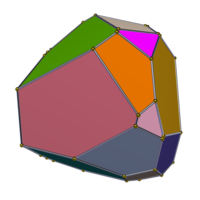
\includegraphics[width=0.8\textwidth]{polytope.png}
	  \end{figure}
      \end{column}
  \end{columns}
\end{frame}

\begin{frame}{UFSC - Use Case}
  \begin{columns}[c]
    \begin{column}{.5\textwidth}

	To try out the real-life application of this optimization problem, we ran an instance of the problem using data from DAE.

    \end{column}
    \begin{column}{.5\textwidth}

	\begin{figure}[h]
	    \centering
	    
\includegraphics[width=0.8\textwidth]{UFSC.pdf}
	\end{figure}

    \end{column}
  \end{columns}
\end{frame}

\begin{frame}{UFSC - Data}
    Data contains the rooms' description and the courses' size and room.

  \begin{columns}[c]
    \begin{column}{.5\textwidth}

	\begin{figure}[h]
	    \centering
	    \colorbox{white}{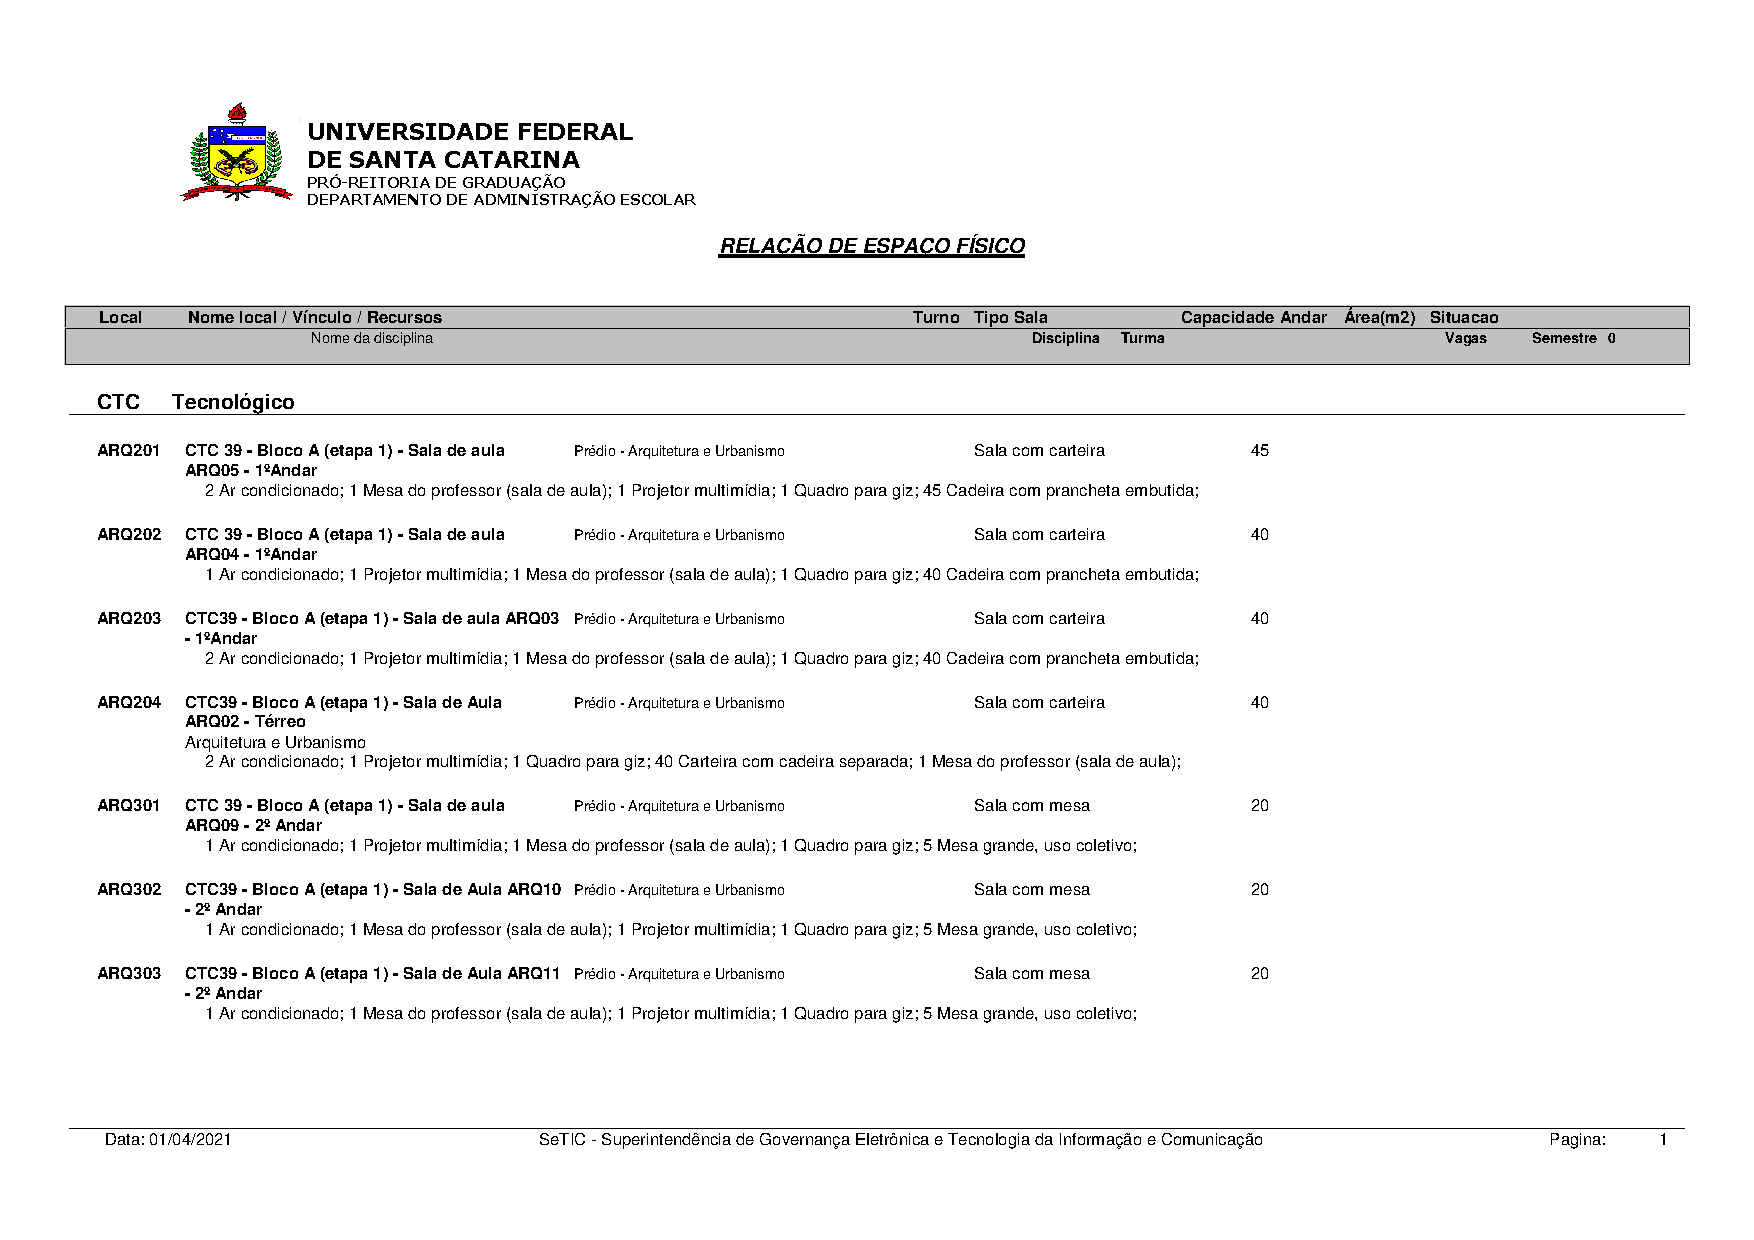
\includegraphics[width=\textwidth]{example-df-rooms.pdf}}
	\end{figure}

    \end{column}
    \begin{column}{.5\textwidth}

	\begin{figure}[h]
	    \centering
	    \colorbox{white}{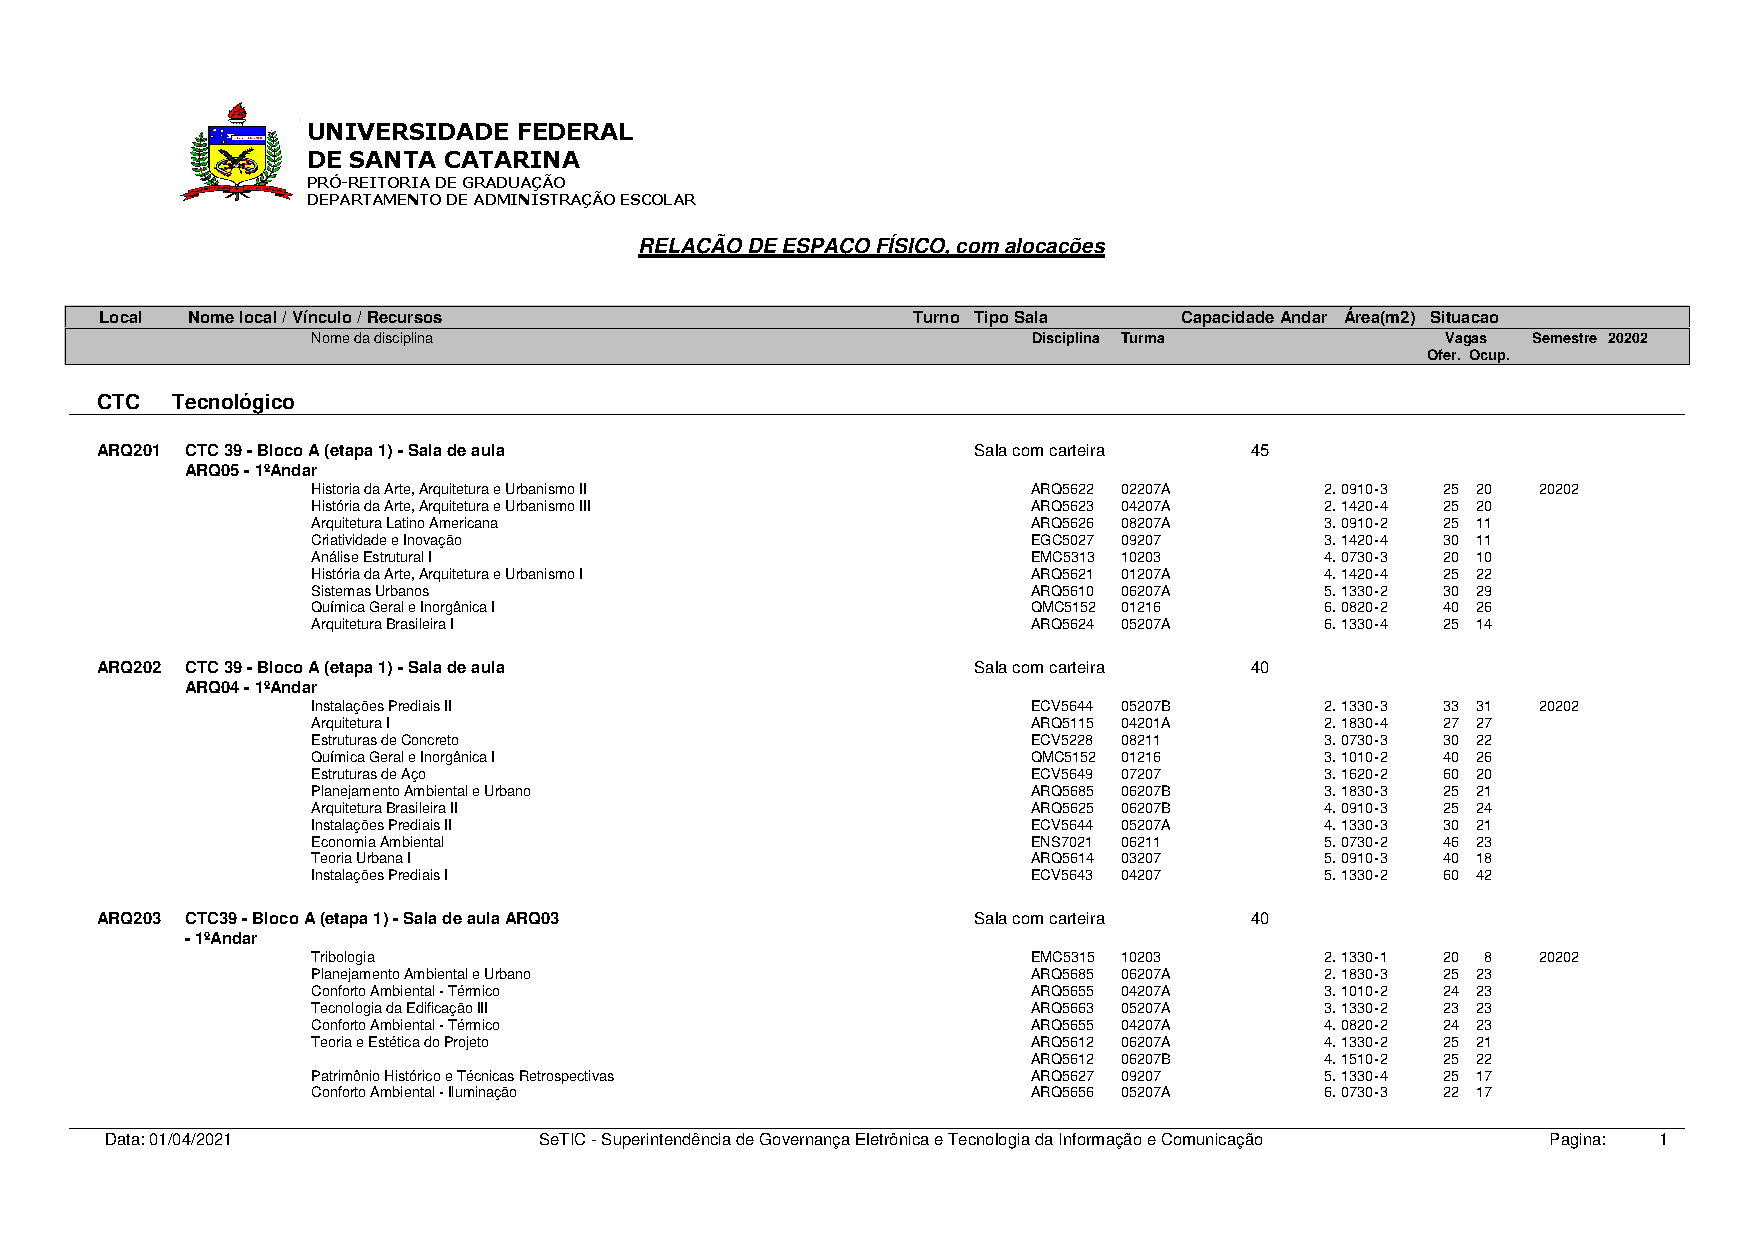
\includegraphics[width=\textwidth]{example-df-classes.pdf}}
	\end{figure}

    \end{column}
  \end{columns}
    
\end{frame}

\begin{frame}{UFSC - Caveats}
    Limitations imposed by us:
    \begin{itemize}
        \item No laboratory room nor any laboratory-requiring courses were included;
	\item All ARQ**** courses were excluded with the rooms used by them;
	\item Limited course-class hierarchy support;
	\item Lectures bigger than the rooms in which they take place were downsized.
    \end{itemize}
\end{frame}

\begin{frame}{UFSC - Formulation Modifications}
    As it was expected, the problem did not fit perfectly to our use case, so some changes in the formulation were necessary due to:
    \begin{enumerate}
	\item Quality measure used was the number of lectures in each pattern;
	\item The room requirement was pattern-based instead of course-based as different lectures from the same course have different number of students enrolled;
        \item $T_r$ is not necessary as all rooms are available full time;
	\item An infeasibility constraint was necessary for modeling.
    \end{enumerate}


\end{frame}
\begin{frame}{UFSC - Formulation Modifications}
    \begin{align*}
	\max_{x_{p,r}} \quad & \sum_{p \in P} \sum_{r\in R} \boldsymbol{w_{p}}x_{p,r} \\
	\textrm{s.t.} \quad & \sum_{p \in P_{r,t}} x_{p,r} \le 1, & r\in R,\,t\in \boldsymbol{T} \\
			    & \sum_{p \in P_l} \sum_{r \in R_p} x_{p,r} \le 1, & l \in L \\
			    & \sum_{p \in P_c} x_{p,r} \le 1, & c \in C,\, r \in R_c \\
			    & x_{p,r} \in \left\{ 0,1 \right\}, & p \in P,\, r\in \boldsymbol{R} \\
			    & \boldsymbol{x_{p,r}=0,} & \boldsymbol{p \in P,\, r \notin R_p} \\
    .\end{align*}
    
\end{frame}

\begin{frame}{UFSC - Solution}
    
  \begin{columns}[c]
    \begin{column}{.35\textwidth}

	\begin{enumerate}
	    \item AMPL model;
	    \item Test through small examples;
	    \item Python data science suite to preprocess the data;
	    \item AMPLPy to bridge the gap;
	    \item Gurobi @ NEOS Server;
	\end{enumerate}

    \end{column}
    \begin{column}{.65\textwidth}
	\lstinputlisting[basicstyle=\tiny]{classroom-slides.mod}
    \end{column}
  \end{columns}
\end{frame}

\begin{frame}{UFSC - Results}

	As we used the number of lectures in each pattern as our quality measure, the objective being equal to the amount of lecture (1012) assures us that all lectures were successfully allocated in a room. \linebreak

    Problem instance (after Gurobi's presolve):
    \begin{itemize}
	\item \textbf{10.433} (+ 9.015) constraints
	\item \textbf{37.316} (+ 5.916) variables
	\item \textbf{7166} simplex iterations
    \end{itemize}
\end{frame}

\begin{frame}{UFSC - Challenges}
    \begin{itemize}
	\item Poor data quality (e.g., courses with more students than seats in the rooms, wrong names/multiple names)
	\item Lack of information about the rooms;
	\item No standard for class groupings;
	\item \textbf{Room preference not clearly defined}.
    \end{itemize}
\end{frame}

\begin{frame}{Conclusion}
This lecture was a brief explanation using a complex modeling approach for the timetabling problem. Solve the universities' timetabling real problem is necessary to add constraints, making it even harder to solve. 
Example of constraints:
    \begin{itemize}
        \item Professors' schedule;
        \item Group together classes from the same curricula;
        \item Adding different classes of lectures (pratical, seminars, theorical);
    \end{itemize}
    

\end{frame}

\begin{frame}{Integer Programming Importance}

In the end, it's important to note that the IP is in our daily lives. We brought the timetabling problem to show how IP is used in practical examples and try to approximate it and the students.

\end{frame}

\contato{E-mail: \\ \url{{ mpacheco.bruno,  pedro_kretz}@gmail.com}}
\capadetras{Thank you!}
%%
%%	Remover o número de páginas do slide com [plain]
%%
\begin{frame}[plain]{Sem número de páginas}
\lipsum[1]
\end{frame}


%%
%%	Você pode usar mais de uma coluna! Inclusão automatizada de imagens com \imagem{arquivo}{label}{legenda}
%%
\begin{frame}{Texto em duas colunas}
  \begin{columns}[c]
    \begin{column}{.5\textwidth}

	O brasão da UFSC pode ser observado na \figurename~\ref{fig:ufsc}.

    \end{column}
    \begin{column}{.5\textwidth}

	\imagem{UFSC.pdf}{fig:ufsc}{Brasão da UFSC.}

    \end{column}
  \end{columns}
\end{frame}


%%
%%	Caixas de texto
%%
\begin{frame}{Caixas de Texto}

\begin{block}{Bloco Normal}
Conteúdo do bloco normal.
\end{block}

\begin{alertblock}{Bloco de Alerta}
Conteúdo do bloco de alerta.
\end{alertblock}

\begin{exampleblock}{Bloco de Exemplo}
Conteúdo do bloco de exemplo
\end{exampleblock}

\end{frame}


%%
%%	Equações
%%
\begin{frame}{Equações}

Observe a Equação \ref{eq:sum}.

% Iniciar ambiente equation
\begin{equation}\label{eq:sum}
\sum_{n=1}^\infty \frac{1}{n^2} = \lim_{n \to \infty} \left( \frac{1}{1^2} + \frac{1}{2^2} + \cdots + \frac{1}{n^2} \right) = \frac{\pi^2}{6}
\end{equation}

Observe as Equações \ref{eq:bhaskara}.

% Iniciar ambiente split dentro de equation para várias linhas
\begin{equation}\label{eq:bhaskara}
\begin{split}
x_1 = \frac{-b + \sqrt{b^2 - 4ac}}{2a} \\
x_2 = \frac{-b - \sqrt{b^2 - 4ac}}{2a}
\end{split}
\end{equation}

\end{frame}


%%
%%	Incluir \capadetras para agradecimentos e contato.
%%
\contato{Contato: \\ \url{{autor1, autor2, autor3}@ufsc.br}}
\capadetras{Obrigado!}

\end{document}
